\documentclass{article}

\usepackage{amsthm}
\usepackage{amsmath}
\usepackage{amsfonts}
\usepackage[margin=0.5in]{geometry}
\usepackage{hyperref}
\usepackage{tikz}
\usepackage{wasysym}

\DeclareMathOperator{\re}{re}
\DeclareMathOperator{\res}{res}
\DeclareMathOperator{\Imag}{Im}
\DeclareMathOperator{\Length}{Length}


\title{\href{https://math.umn.edu/sites/math.umn.edu/files/exams/complexanalysis_fall2020.pdf}{Fall 2020 Complex Analysis Preliminary Exam}}
\author{University of Minnesota}
\date{}
\begin{document}
\maketitle

This is a verbatim transcription of an exam which received a score of 89/100. Mistakes are intentionally included.

\begin{enumerate}

	\item	Give a conformal mapping from the half-disk $H = \{z: |z| < 1 \text{ and } \Imag(z)>0\}$ to the upper half-plane
	$\mathfrak{h} = \{ z : \Imag (z) > 0 \}$.
	
	\begin{proof}
		Define $f: H \rightarrow D$ by $z \mapsto z^2$ where $D$ is the unit disk, slit along $\mathbb{R}_{\geq 0}$.
		Define $g: D \rightarrow \mathfrak{h}$ by the Cayley map $\frac{iz + i}{-z+1}$.
		We clam [sic] $g \circ f$ is the desired mapping. Since $\arg (z) \in (0, \pi) $ for all $z \in H$ and $|z| < 1$, then
		$\arg(z) \in (2\cdot 0, 2\pi)$ and $|z^2| < 1^2$, so $f$ is inded [sic]. Note $f^\prime(z) = 2z$ is only zero at 
		$z=0$, but $0 \not \in H$, so it is indeed conformal.
		The derivatve [sic] of $g$ is $g^\prime = \frac{2i}{(1-z)^2}$, which is nonzero on its domain, 
		which is $\mathbb{C} \backslash \{1\}$. Moreover $f(H) \not \ni 1$.
		Thus, $g^\prime(f) \neq 0$, and so the composition $g \circ f$ is conformal.
		
		To see $f$ is onto, let $z \in D.$ Then $\arg(z) \in (0, 2\pi)$ and $|z| \leq 1$ so 
		$|\sqrt{z}| \leq 1$ (choosing the principal branch of $\sqrt{\bullet}$) and $\arg(\sqrt{z})$ is in $(0, \pi)$ so
		$f$ is onto. To see $g$ is onto, note that its explicit inverse is $\frac{z-i}{z+i}$, which takes points closer 
		to $i$ than to $-i$ (i.e. the upper half plane) to a point in the slit disk.
	\end{proof}
	
	\item Write three (non-zero) terms of the Laurent expansion of $f(z) = \frac{1}{z(z-1)(z-2)}$ centered at $1$ and convergent in 
	$0 < |z-1| < 1$.
	
	\begin{proof}
		First, apply the change of coordinates $w = z-1$. Then we can write $f(z) = f(w+1) = \frac{1}{w(w+1)(w-1)}$ 
		and we seek the Laurent expansion of $f(w+1)$ centered at $w=0$. Using geometric series, this becomes
		\[ \frac{1}{w(w+1)(w-1)} = \frac{1}{w} \left ( - \sum_{n \geq 0} w^n \right ) \left ( \sum_{n \geq 0} (-w)^n \right). \]
		Since $\frac{1}{w-1} = - \sum_{n \geq 0} w^n$ for $|w| < 1$, and 
		$\frac{1}{w+1} = \frac{1}{1-(-w)} = \sum_{n \geq 0} (-w)^n$ for $|w| < 1$. Then multiplying, we get
		
		\begin{align*}
			f(w+1) &= \frac{1}{w} (-1)(1) + \frac{1}{w}(-w + (+w))\\
				   &\;+ \frac{1}{w} ( -w^2 + (-w)(-w) + (-w)^2) \\
				   &\;+ \frac{1}{w} (-w^3 + (-w^2)(-w) + (-w)(-w)^2 + (-w)^3)\\
				   &\;+ \frac{1}{w} (-w^4 + (-w^3)(-w) + (-w^2)((-w)^2) + (-w)(-w)^3 +(-w)^4)\\
				   &\;+ \cdots\\
				   &= \frac{-1}{w} + 0 + w + 0 +(-1)w^3 + \cdots 
		\end{align*}
		
		Undoing our change of coordinates, we get
		\[ f(z) = \frac{-1}{z-1} + (z-1) - (z-1)^3 + \cdots \]
		Since it converged for $|w|<1$, it also converges for $|z-1| < 1$.
	\end{proof}
	
	\item Let $f$ be an entire function taking real values on the real line. 
	Show that, for all complex $z$, $\overline{f(z)} = f(\overline{z})$.
	
	\begin{proof}
		The Schwarz reflection principle states that if $\Omega$ is a region which is symmetric about the real-axis, and
		$f$ is a function hollomorphic [sic] in $\Omega \cap \{z: \Imag(z) > 0\}$ which has a continuation onto 
		$\mathbb{R} \cap \Omega$ and that continuation is real-valued, then there is a holomorphic function $F$ on 
		$\Omega$ st $F=f$ on $\Omega \cap \{ z : \Imag(z) > 0\}$ and moreover, $F(z) = \overline{f(\overline{z})}$.
		Note that we may take $\Omega = \mathbb{C}$ and the continuation to be just the real values on $\mathbb{R}$
		which we know it takes. 
		Then $\overline{F(z)} = \overline{f(z)} = \overline{\overline{f(\overline{z})}} = f(\overline{z}).$
	\end{proof}
	
	\item Classify entire functions $f$ such that there is a constant (possibly depending on $f$) such that
	$|f(z)| \leq C \cdot \log (1 + |z|)$.
	
	\begin{proof}
	If $f$ is entire it admits a powder [sic] series representaton [sic] centered at $0$, so
	\[ f(z) = \sum_{n \geq 0} \alpha_n z^n\]
	
	Cauchy's inequality tells us that on a circle of radius $R$ about $z_0$, call it $\gamma_R$, that
	\[ | f^{(n)} (z_0) |\leq \frac{n! \max_{z \in \gamma_R} |f(z)|}{R^n} \]
	to extract the coefficients $\alpha_n$ from $f$ note that 
	\[ \alpha_n = f^{(n)}(0)/n!\]
	so taking $z_0 = 0$, we get 
	\[ | \frac{f^{(n)}(0)}{n!}| = |\alpha_n| = \leq \frac{\max_{z \in \gamma_R} |f(z)|}{R^n} \] 
	The provided bound tells us that $\max_{C_R} |f(z)| \leq C \cdot \log (1+R)$ and so
	\[ | \alpha_n | \leq \frac{C \log (1+R)}{R^n} \]
	This is independent of $R$, so we take the limit 
	\[ \lim_{R \rightarrow \infty} \frac{C log(1+R)}{R^n} = \lim_{R \rightarrow \infty} \frac{C \frac{1}{1+R}}{nR^{n-1}} \;\;\; \text{(by L'H\^opitals [sic] rule)}\]
	which vanishes for $n \geq 1$. So $f$ is constant, but we can do better. If $f$ is constant,
	$f(z) \equiv f(0)$. So $|f| \leq C \log(1+|0|) = 0$, so $f$ is identically 0 on $\mathbb{C}$.
	\end{proof}
	
	\item Evaluate $\int_0^\infty \frac{x^{1/2}}{1+x^2} dx$
	
	\begin{proof}
	We compute by passing to $\mathbb{C}$ and defing [sic] $f(x) = \frac{z^{(1/4)}}{1+z^2}$.
	Choose $z^{1/4}$ to be defined using the branch cut from the origin through $-i$. In particular
	$f$ is not defined at zero. Define the curve $\gamma_{R,\epsilon}$ for $R>1$, $0 < \epsilon < 1$ as the
	union of the circles of radii $R, \epsilon$ with counter clockwise and clockwise orientations respectively,
	and connect them along $[-R, \epsilon]$\footnote{This should be $-\epsilon$.} and $[\epsilon, R]$, to get
	
		\begin{center}
		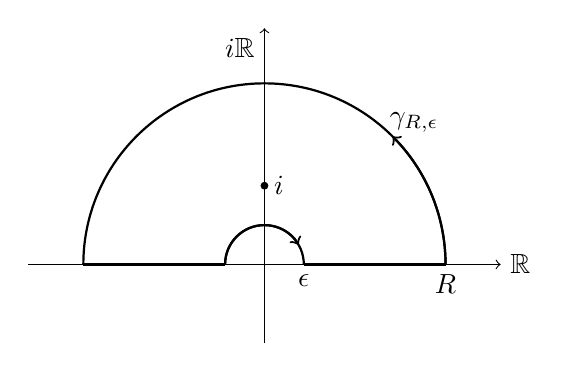
\begin{tikzpicture}
			%\draw[step=1cm,gray,very thin] (-2.9,-0.9) grid (2.9,2.9);
			\draw[thin,->] (0,-1) -- (0,3); 
			\draw[thin,->] (-3,0) -- (3,0);
			
			\node[anchor = north east] at (0,3) {$i \mathbb{R}$};
			\node[anchor = west] at (3,0) {$ \mathbb{R}$};
			
			\node[fill = black, inner sep=1pt, circle] at (0,1) {};
			\node[anchor = west] at (0,1) {$i$};
			
			\node[anchor = north] at (2.3,0) {$R$};
			\node[anchor = north] at (.5,0) {$\epsilon$};

			
			\node at (1.9,1.8) {$\gamma_{R,\epsilon}$};
			
			\draw[thick, ->] (2.3,0) arc (0:45:2.3) ;
			\draw[thick] (2.3,0) arc (0:180:2.3) ;
			
			\draw[thick, ->] (-.5,0) arc (0:-150:-.5);
			\draw[thick] (-.5,0) arc (0:-180:-.5);
			\draw[thick] (0.5,0)--(2.3,0);
			\draw[thick] (-0.5,0)--(-2.3,0);
		\end{tikzpicture}
		\end{center}
	
	The residue theorem states that 
	\[ \int_{\gamma_{R,\epsilon}} f dz = 2\pi i \sum_{\substack{\text{poles}\\\text{inside}\\ \gamma_{R,\epsilon}}} \res_{z_0}(f) \]
	
	The only pole of $f$ inside $\gamma_{R,\epsilon}$ is the one at $z=i$ which is simple. So we may compute
	\begin{align*}
		\res_i (f) &= \lim_{z \rightarrow i} (z-i) f(z) \\
		&= \frac{i^{1/4}}{2i}
	\end{align*}
	and so $\int_{\gamma_{R,\epsilon}} f dz = \pi i^{1/4}$. Now observe that, if $C_R^+$ represents the 
	circle of radius $R$ in the upper half plane, then 
	
	\[\int_{\gamma_{R,\epsilon}} f dz = \int_{C_R^+} f dz - \int_{C_\epsilon^+} f dz + \int_{-R}^{-\epsilon} f dz + \int_\epsilon^R f dz \]
	
	where we subtract the integral on $C_\epsilon^+$ because of the choice of orientation.
	We will show that the circular parts vanish in the limit, since $\int_{\gamma_{R,\epsilon}} f dz$ was independent of $R,\epsilon.$
	
	The estimation lemma gives the bound
	\begin{align}
		\left | \right | & \leq \Length(C^+_R) \max_{|z| = R} |f(z)| \nonumber\\
		&= \pi R \max_{|z| = R} \left | \frac{z^{1/4}}{z^2+1} \right | \nonumber\\
		&= \pi R^{5/4} \max_{|z| = R} \left | \frac{1}{z^2+1} \right | \label{eqn:Star}
	\end{align}
	
	Note that $\left | \frac{1}{z^2+1} \right |$ is maximized when $|z^2 - (-1)|$ is minimized.
	Since $|z| = R$ is closes to $-1$ at $R = -z$, we can write
	\[ (\ref{eqn:Star}) = \pi R^{5/4} \frac{1}{(-R)^2 + 1} \]
	Since $5/4 < 2$, (\ref{eqn:Star}) vanishes upon taking $R \rightarrow \infty$.
	
	The same computation shows that 
	\[ \left | \int_{C^+_{\epsilon}} f(z) dz \right | \leq \pi \epsilon^{5/4}/(\epsilon^2+1)\]
	as $\epsilon \rightarrow 0$, the numerator vanishes and the denominator $\rightarrow 1$.
	So
	\[ \pi i^{1/4} = \int_{\gamma_{\infty, 0}} f(z) dz = \int_{-\infty}^0 f dz + \int_0^\infty f dz \]
	A change of variables gives us 
	\[ \int_{-\infty}^0 f(z) dz = \int_{\infty}^0 f(-z) (-1) dz = \int_0^\infty f(-z) dz.\]
	But $f(-z) = (-1)^{1/4} f(z)$ so we get 
	\[ \pi i^{1/4} = \left ( (-1)^{1/4} _1 \right ) \int_0^\infty f(z) dz \]
	so 
	\begin{align*}
		\int_0^\infty f(z) dz = \pi i^{1/4}/ ((-1)^1/4 + 1) &= \pi \frac{i^{1/4}}{i^{1/2} +1}\\
		&=\pi/(i^{1/4} + i^{-1/4})
	\end{align*}
	But note that 
	\[i^{1/4} = \cos (\pi/8) + i \sin (\frac{\pi}{8})\]
	\[i^{-1/4} = \cos (\pi/8) - i \sin (\pi/8) \]
	so
	\[ \int_0^\infty f(z) dz = \boxed{\frac{\pi}{2 \cos(\pi/8)}}\]
	
	\end{proof}
	
	\item Let $f, g$ be holomorphic functions on $\{z : |z| < 2\}$ with $f$ nonvanishing on $|z| - 1$. 
	Show that for all sufficiently small $\epsilon > 0$ the function $f + \epsilon g$ has the same number of zeros inside $|z| = 1$ 
	as does $f$.
	
	\begin{proof}
	Rouche's theorem tells us that if $f,h$ holomorphic on and inside (eg) the unit disk, and $|f|>|h|$ on
	all of the boundary $|z|=1$, then $f, f+h$ have the same number of zeros inside the unit disk.
	Since the boundary is compact (closed and bounded), $|f|,|g|$ achieve both a maximum and a 
	minimum on $|z|=1$. Let $m:= \min_{|z|=1} |f|$ and $M:= \max_{|z|=1} |g|$. Then $|\frac{g}{M}| \leq 1$
	and so 
	\[ \left | \frac{mg}{M} \right | \leq |f| \;\;\; \text{ on } |z|=1.\]
	then take $\epsilon < m/M$ and $h = \epsilon g$ in the statement of Rouche's theorem.
	\end{proof}
	
	\item Describe all harmonic functions on the punctured unit disk $\{z : 0 < |z| < 1\}$, continuous on the punctured closed disk
	$\{z: 0 < |z| \leq 1\}$ whose restriction to $\{z: |z| = 1\}$ is the zero function.
	
	\begin{proof}
		The maximum modulus principle tells us that $f$ is holomorphic on $|z|<1$, then $|f|$ does not 
		attain a maximum on $|z| < 1$, and so any maximum must occur on $|z| = 1$. If a function $f$
		is harmonic on $\{z: 0 < |z| < 1\}$, it admits an analytic continuation on $\{z: |z| \leq 1\}$ 
		call this continuation $F$. Then $|F|$ attains its maximum on $|z|=1$. Since $F=0$ on $|z|=1$,
		$|F| \leq 0$ on the whole punctured disk, and so $f$ must be identically $0$.
	\end{proof}
	
	\item Show that the curve $z^3+w^3=1$ has genus 1.
	
	\begin{proof}
		The degree-genus formula tells us that if we have a smooth, irreducible plane curve, then 
		its genus is 
		\[ \frac{(d-1)(d-2)}{2}\]
		where $d$ is the degree of the curve. To see that the given curve is smooth, homogenize
		so we are dealing with $p = z^3+w^3-u^3 = 0$. The partial derivatives 
		$\frac{\partial}{\partial z} p = 3z^2,
		\frac{\partial}{\partial w} p = 3w^2,
		\frac{\partial}{\partial u} p = -3u^2$
		are only simultaneously $0$ when (in homogeneous coordinates) we are at the point 
		$[0:0:0]$. But that point is never on our given curve which looks like
		$[* : * : 1]$. To see it is irreducible, note that $-w^3+1$ has zeros at the 3 third roots of unity,
		which are distinct, so it is squarefree. Hence, we apply the formula with $d=3$ to get 
		d$\frac{(3-1)(3-2)}{2} = 1$
		\end{proof}
		
\end{enumerate}


\end{document}